\chapter{Introduction}
\label{cha:introduction}

\section{Motivation}
\label{sec:motivation}

Many of us have been struck by the inherent beauty of animals moving collectively; starlings gathering at dusk in huge numbers to perform the most mesmerising of ballets, the entire flock moving as if some fluid object; fish forming tight milling structures in defence against predation, changing direction in the blink of an eye and with a flash of silver. At different length scales, and in both the living and non-living domains, startling examples of collective behaviours have been observed \citep{parrish99}.

\begin{figure}[!htbp]
	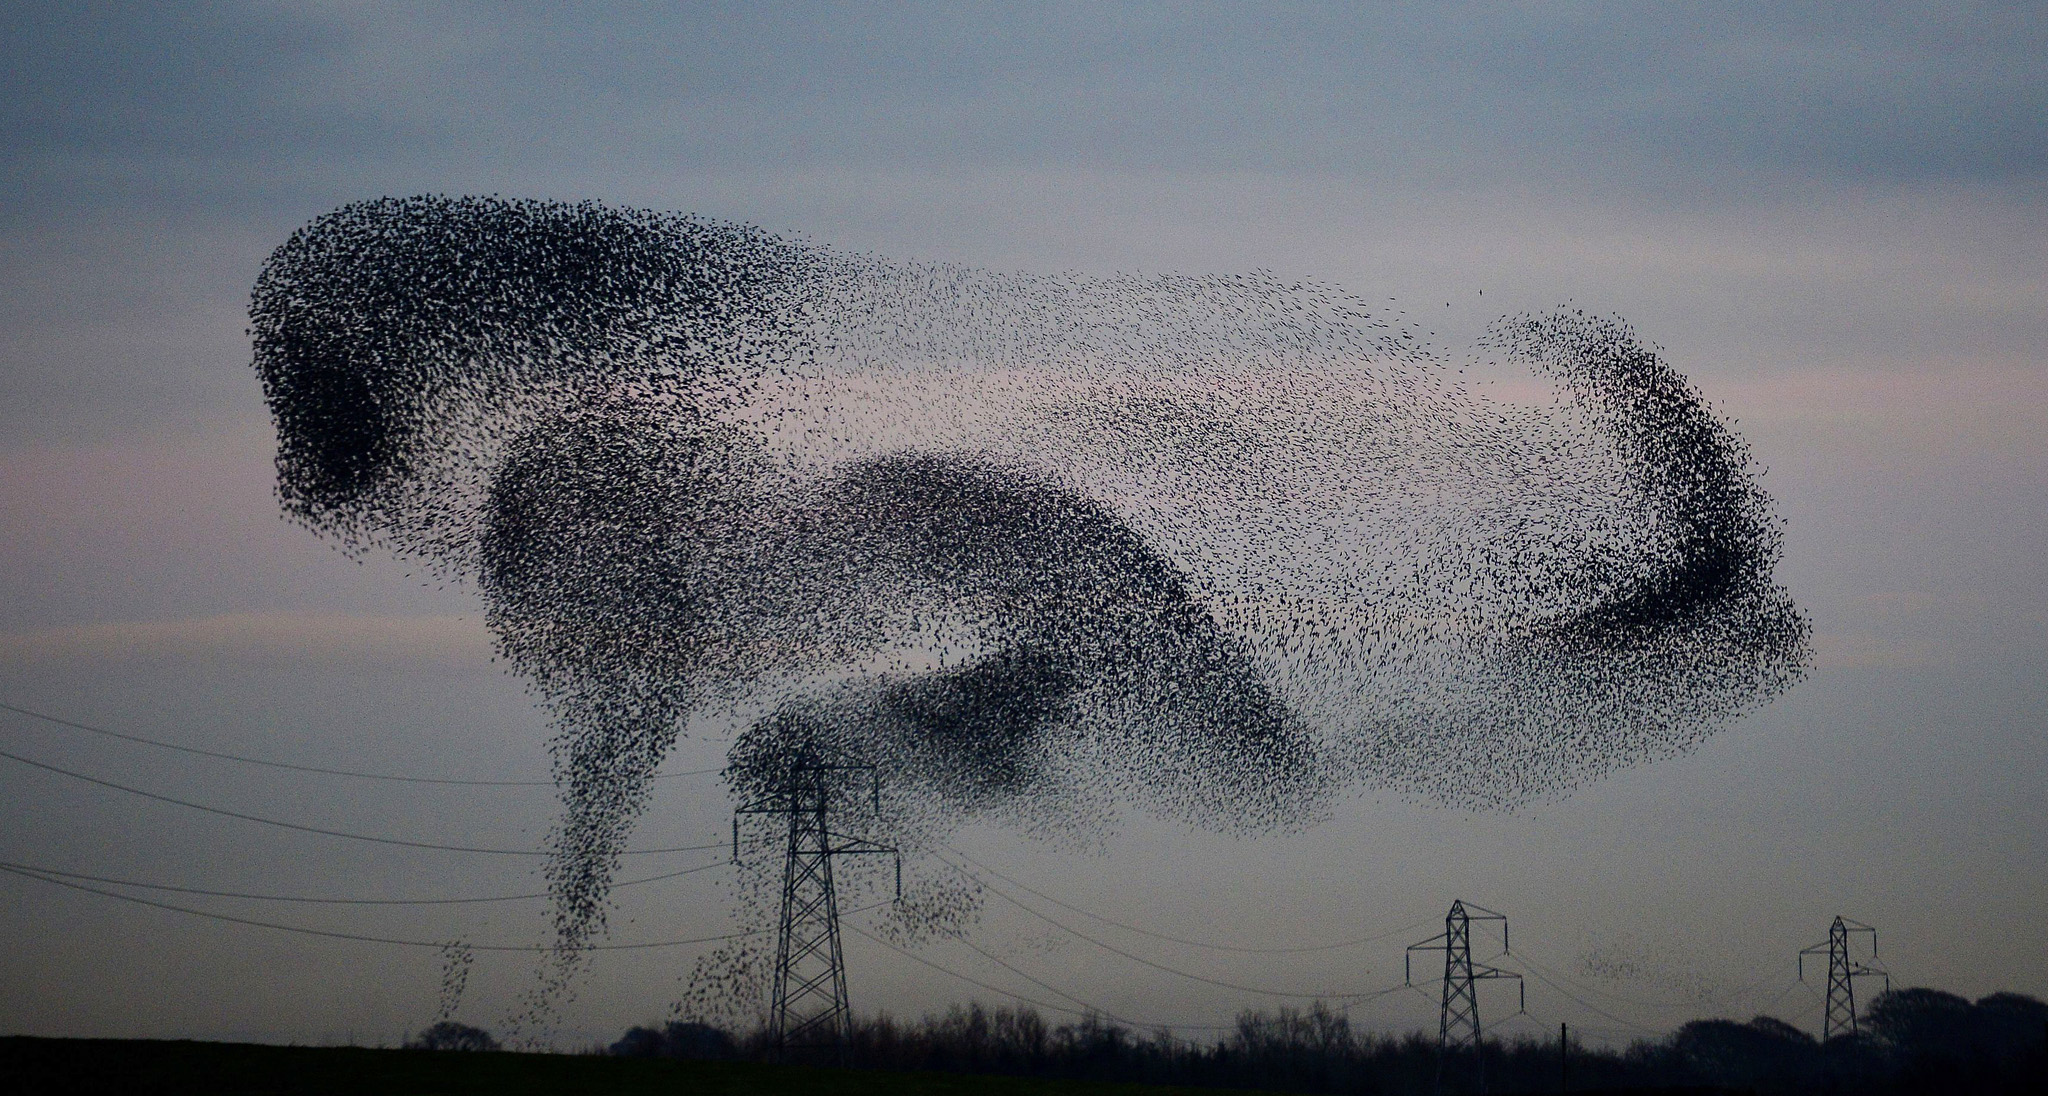
\includegraphics[width=\textwidth]{murmuration.jpg}
	\caption{A particularly startling example of a starling murmuration, captured near Gretna in the Scottish Borders. Photograph: Owen Humphreys/PA.}
	\label{fig:murmuration}
\end{figure}

Over the years collective behaviour has become a thriving topic of multidisciplinary research, capturing the imaginations of physicists \citep{vicsek95}, biologists \citep{couzin02}, mathematicians \citep{lukeman10} and statisticians \citep{mann11}. Our understanding has evolved significantly from early suggestions that collective behaviour results from thought-transference and telepathy between individuals \citep{selous31}. Though we can often explain why animal aggregations are evolutionary advantageous \citep{giardina08}, much less is known about how these structures are formed and maintained.

Much work has been invested in developing theoretical models which seek to explain emergent behaviour by interactions at an individual level. Such models have shown that individual interactions are sufficient to produce group-level structures. Many different simulations, implementing disparate interaction rules, are able to produce behaviour reminiscent of real flocking systems. However, these models have largely only been verified with comparison to empirical observation at a qualitative level, and a thorough quantitative comparison between field data and theory has been lacking.

In recent years technological and methodological advances have made it possible to capture the movements of large groups of animal aggregates \citep{ballerini08}. With this data, it is only now that we are in a position to make a robust comparison between model predictions and real-world observations.

\section{Overview of thesis}
\label{sec:overview_of_thesis}

We begin this thesis by giving the reader a review of the literature surrounding collective behaviour. Important results and ideas of the field are introduced and discussed. After relaying the main results from the literature we discuss open problems and the future of research in the field. Finally, we explain how our work will fit into the current research landscape using techniques from Bayesian statistics.

Chapter \ref{cha:bayes_intro} will introduce the reader to the field of Bayesian statistics. Important results, techniques and algorithms from the field will be outlined as well as problems that the practitioner may encounter. 